\documentclass{exam}
\usepackage[utf8]{inputenc}
\usepackage{lmodern}
\usepackage{microtype}

% \usepackage[parfill]{parskip}
\usepackage[dvipsnames]{xcolor}
\usepackage{amsmath}
\usepackage{amsfonts}
\usepackage{amsthm}
\usepackage{siunitx}
\DeclareSIUnit\year{yr}
\DeclareSIUnit\foot{ft}
\DeclareSIUnit\litre{\liter}

\usepackage{skull}

\usepackage{pgfplots}
\usepgfplotslibrary{polar}
\pgfplotsset{compat=1.11}
\usepgfplotslibrary{statistics}
\usepackage{graphicx}
\usepackage{sidecap}
\sidecaptionvpos{figure}{c}
\usepackage{float}
\usepackage{gensymb}
\usepackage{tkz-euclide}
\usetkzobj{all}
\usepackage{commath}
\usepackage{hyperref}
\usepackage{enumitem}
\usepackage{wasysym}
\usepackage{multicol}
\usepackage{mathtools}
\usepackage{tcolorbox}
\usepackage{tabularx}
\usepackage[version=4]{mhchem}
\usepackage{changepage}
\usepackage{listings}
\lstset{basicstyle=\ttfamily\linespread{0.8}\small}

\renewcommand*{\thefootnote}{\fnsymbol{footnote}}

\newtheorem*{thm}{Theorem}
\newtheorem*{iden}{Identity}
\newtheorem*{lemma}{Lemma}
\newtheorem{obs}{Observation}
\theoremstyle{definition}
\newtheorem*{defn}{Definition}
\newtheorem*{ex}{Example}
\newtheorem{con}{Construction}
\newtheorem*{alg}{Algorithm}

\newtheoremstyle{break}
  {\topsep}{\topsep}%
  {\itshape}{}%
  {\bfseries}{}%
  {\newline}{}%
\theoremstyle{break}
\newtheorem*{bthm}{Theorem}

% russian integral
\usepackage{scalerel}
\DeclareMathOperator*{\rint}{\scalerel*{\rotatebox{17}{$\!\int\!$}}{\int}}

% \DeclareMathOperator*{\rint}{\int}

\pgfplotsset{vasymptote/.style={
    before end axis/.append code={
        \draw[densely dashed] ({rel axis cs:0,0} -| {axis cs:#1,0})
        -- ({rel axis cs:0,1} -| {axis cs:#1,0});
    }
}}

% \pointsinrightmargin
\boxedpoints
\pointname{}

\newcommand{\questioA}{\question[\texttt{\textbf{\color{Cerulean} A}}]}
\newcommand{\questioM}{\question[\texttt{\textbf{\color{PineGreen} M}}]}
\newcommand{\questioE}{\question[\texttt{\textbf{\color{WildStrawberry} E}}]}
\newcommand{\questioS}{\question[\texttt{\textbf{\color{Goldenrod} S}}]}
\newcommand{\questioO}{\question[\texttt{\textbf{\color{BurntOrange} O}}]}

\newcommand{\parA}{\part[\texttt{\textbf{\color{Cerulean} A}}]}
\newcommand{\parM}{\part[\texttt{\textbf{\color{PineGreen} M}}]}
\newcommand{\parE}{\part[\texttt{\textbf{\color{WildStrawberry} E}}]}
\newcommand{\parS}{\part[\texttt{\textbf{\color{Goldenrod} S}}]}
\newcommand{\parO}{\part[\texttt{\textbf{\color{BurntOrange} O}}]}

\newcommand{\subparA}{\subpart[\texttt{\textbf{\color{Cerulean} A}}]}
\newcommand{\subparM}{\subpart[\texttt{\textbf{\color{PineGreen} M}}]}
\newcommand{\subparE}{\subpart[\texttt{\textbf{\color{WildStrawberry} E}}]}
\newcommand{\subparS}{\subpart[\texttt{\textbf{\color{Goldenrod} S}}]}
\newcommand{\subparO}{\subpart[\texttt{\textbf{\color{BurntOrange} O}}]}

\newcommand{\mainHeader}[2]{\section*{NCEA Level 2 Mathematics\\#1. #2}}
\newcommand{\mainHeaderHw}[2]{\section*{NCEA Level 2 Mathematics (Homework)\\#1. #2}}
\newcommand{\seealso}[1]{\begin{center}\emph{See also #1.}\end{center}}
\newcommand{\drills}[1]{\begin{center}\emph{Drill problems: #1.}\end{center}}
\newcommand{\basedon}[1]{\begin{center}\emph{Notes largely based on #1.}\end{center}}

\begin{document}

\mainHeaderIntg{18}{Substitution}
Recall that the \textbf{chain rule} for differentiation is given by
\begin{displaymath}
  \od{}{x} [f(g(x))] = f'(g(x)) g'(x).
\end{displaymath}

Since integration is (in some sense) the inverse of differentiation, we can write (by applying the fundamental theorem of calculus)
\begin{displaymath}
  \rint f'(g(x)) g'(x) \dif{x} = f(g(x)) + C.
\end{displaymath}

For a mnemonic, we can let $ u = g(x) $. Then $ \dif{u} = g'(x) \dif{g} $\footnote{This rearrangement is not rigorous, but it works.}
and so, by the rule we just wrote down, we have
\begin{displaymath}
  \rint f'(g(x)) g'(x) \dif{x} = \rint f'(u) \dif{u} = f(u) + C = f(g(x)) + C.
\end{displaymath}

In Leibniz notation, we have
\begin{displaymath}
  \rint f'(g(x)) g'(x) \dif{x} = \rint \od{f}{g} \od{g}{x} \dif{x} = \rint \od{f}{g} \dif{g} = \rint f'(g) \dif{g} = f(g) + C = f(g(x)) + C,
\end{displaymath}
and so one can intuitively think about this (here we substitute $ g $ out) as the cancellation of differentials underneath an integral sign.

This rule, which gives us a kind of chain rule for integration, is called \textbf{substitution}, or the \textbf{inverse chain rule}. It
can be thought of as a change in coordinate system from an $ x$-based system to one based on $ u $, and we have to `resize' our area based
on how much $ u $ stretches the coordinate system compared to $ x $ --- and this `stretch factor' is simply $ \od{u}{x} $.

\begin{ex}
  For example, consider $ \rint_1^2 2x(x^2 + 1) \dif{x} $; we are finding the area shown here between the dotted lines.
  \begin{center}
    \fbox{\begin{tikzpicture}
      \begin{axis}[
        axis lines = center,
        xlabel = $ x $,
        ylabel = {$ y $},
        ymax = 40, ymin = -40,
      ]
        \addplot[domain = -3:3, color = red, samples = 100] {2*x*(x^2 + 1)};
        \draw[style=dotted] (1,-40) -- (1,40);
        \draw[style=dotted] (2,-40) -- (2,40);
      \end{axis}
    \end{tikzpicture}}
  \end{center}
  Let us make the substitution $ u = x^2 + 1 $, so $ \od{u}{x} = 2x $ and our integral becomes
  \begin{displaymath}
    \rint_1^2 2x(x^2 + 1) \dif{x} = \rint_{u^{-1}(2)}^{u^{-1}(5)} \od{u}{x} u(x) \dif{x} =  \rint_2^5 u \dif{u}.
  \end{displaymath}
  We can graph our region of integration again.
  \begin{center}
    \fbox{\begin{tikzpicture}
      \begin{axis}[
        axis lines = center,
        xlabel = $ u $,
        ylabel = {$ y $},
        ymax = 6, ymin = -6,
      ]
        \addplot[domain = -6:6, color = red, samples = 100] {x};
        \draw[style=dotted] (2,-6) -- (2,6);
        \draw[style=dotted] (5,-6) -- (5,6);
      \end{axis}
    \end{tikzpicture}}
  \end{center}
  This new coordinate system, which is $ 2x $ times as large as the older one, is much simpler to integrate inside!
\end{ex}

\begin{exs}\leavevmode
  \begin{enumerate}
    \item Suppose we wish to find $ \rint \sin x \cos x \dif{x} $. Then let $ u = \sin x $, so $ \dif{u} = \cos x \dif{x} $
          and
          \begin{displaymath}
            \rint \sin x \cos x \dif{x} = \rint u \dif{u} = \frac{1}{2} u^2 + C = \frac{1}{2} \sin^2 x + C.
          \end{displaymath}
    \item In this case, we also could have used a trigonometric identity.
          Suppose we wish to find $ \rint xe^{x^2} \dif{x} $. We can let $ u = x^2 $, and then $ du = 2x \dif{x} \Rightarrow \dif{x} = \frac{du}{2x} $.
          Hence:
          \begin{displaymath}
            \rint xe^{x^2} \dif{x} = \rint \frac{1}{2} e^u \dif{u} = \frac{1}{2} e^u + C = \frac{1}{2}e^{x^2} + C.
          \end{displaymath}
    \item Suppose we wish to find $ \rint \frac{4}{x} (\ln x)^3 \dif{x} $. We let $ u = \ln x $, and then $ \dif{u} = \frac{\dif{x}}{x} $.
          Hence:
          \begin{displaymath}
            \rint \frac{4}{x} (\ln x)^3 \dif{x} = 4\rint u^3 \dif{u} = u^4 + C = (\ln u)^4 + C.
          \end{displaymath}
  \end{enumerate}
\end{exs}

\subsection*{Questions}
\begin{questions}
  \questioA Find the following indefinite integrals.
    \begin{multicols}{2}
    \begin{parts}
      \part $ \rint \sin 2x \dif{x} $
      \part $ \rint (4x - 44)^{2019} \dif{x} $
      \part $ \rint 4x \sqrt{x^2 + 3} \dif{x} $
      \part $ \rint (3t - 4)^2 \dif{x} $
      \part $ \rint \frac{x}{x^2 + 1} \dif{x} $
      \part $ \rint \frac{2}{4x + 3} \dif{x} $
      \part $ \rint e^{2x + 1} \dif{x} $
      \part $ \rint \sec 4x \tan 4x \dif{x} $
      \part $ \rint 2\cos x + \sin 2x \dif{x} $
      \part $ \rint -2x\csc^2 (3x^2) \dif{x} $
      \part $ \rint \frac{3}{x^3} - \frac{4}{x + 1} \dif{x} $
      \part $ \rint e^{x/2} + \frac{2}{x} \dif{x} $
      \part $ \rint x^2 \sec^2 x^3 + 9 \dif{x} $
      \part $ \rint -\csc (\tan x) \cot (\tan x) \sec^2 x \dif{x} $
      \part $ \rint \frac{\cos x - \sin x}{\cos x + \sin x} \dif{x} $
      \part $ \rint \frac{2017}{x\ln x} \dif{x} $
    \end{parts}
    \end{multicols}
  \questioM By using the substitution $ x = \sin \theta $, find
            \begin{displaymath}
              \rint \frac{1}{\sqrt{1 - x^2}} \dif{x}.
            \end{displaymath}
  \questioM Compute the following definite integrals:
    \begin{parts}
      \part $ \rint^1_0 xe^{-x^2} \dif{x} $
      \part $ \rint^{\pi/3}_{-\pi/3} x^4 \sin x \dif{x} $ (hint: no substitution is required)
      \part $ \rint^1_0 \cos(\pi t/2) \dif{t} $
      \part $ \rint^1_0 (3t - 1)^{50} \dif{t} $
      \part $ \rint^1_0 \sqrt[3]{1 + 7x} \dif{x} $
      \part $ \rint^1_0 \frac{\dif{x}}{1 + \sqrt{x}} \dif{x} $
      \part $ \rint^2_{-1} x(x-1)^3 \dif{x} $
      \part $ \rint^3_0 x\sqrt{1 + x^2} \dif{x} $
    \end{parts}
  \questioM Find the area enclosed by the curve $ y = 4 \sin 3x \cos x $ and the $ x-$axis from $ x = 0 $
            to $ x = \frac{\pi}{3} $.
  \questioE Find $ k $ such that $ \rint^k_0 e^{2x} \dif{x} = 40 $.
  \questioE Calculate the area enclosed by the curve $ y = \frac{3x - 2}{x + 4} $ and the lines $ y = 0 $, $ x = 1 $,
            and $ x = 5 $.
  \questioE Find the area between the curves $ y = \sin^2 kx $ and $ y = \cos^2 kx $ shaded below.
            \begin{center}
              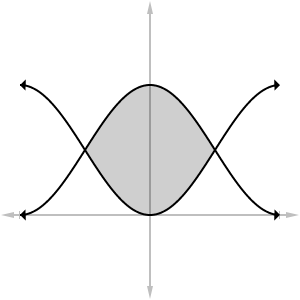
\includegraphics[width=0.3\textwidth]{int4}
            \end{center}
  \questioM Find $ \rint \tan \theta \dif{\theta} $ and $ \rint \cot \theta \dif{\theta} $.
  \questioA Complete the following working:
    \begin{align*}
      \rint \sec x \dif{x} &= \rint \sec x \frac{\sec x + \tan x}{\sec x + \tan x} \dif{x}\\
                           &= \rint \frac{\dots}{\sec x + \tan x} \dif{x}\\
                           \text{Let $ u = \dots $}\\
                           &= \rint \frac{1}{\dots} \dif{u}\\
                           &= \dots
    \end{align*}
  \questioM Show that
    \begin{displaymath}
      \rint x^4 \sin x \dif{x} = 4x(x^2 - 6x) \sin x - (x^4 - 12x^2 + 24) \cos x + C.
    \end{displaymath}
  \questioM If $ y = x \sqrt{\sin x^3 + \cos x^3} $, find $ \pi \rint^1_0 y^2 \dif{x} $.
  \questioM The velocity of a particle at time $ t $ is given by $ v = \frac{\cos(\sqrt{2t + 1})}{\sqrt{2t + 1}} $.
            What is the position of the particle at time $ t = 5 $, given that $ x(0.5) = 0 $? (Recall that $ v = \od{x}{t} $.)
  \questioS Evaluate $ I = \rint^{\pi/2}_0 \frac{\sqrt{\sin x}}{\sqrt{\sin x} + \sqrt{\cos x}} \dif{x} $ [\textit{Hint: use the
            substitution $ x = \frac{\pi}{2} - u $ and add the result to the original integral.}]
  \questioS Scholarship 1999:
    \begin{parts}
      \part Evaluate $ \rint \cos^5 x \dif{x} $ using the substitution $ t = \sin x $.
      \part
        \begin{subparts}
          \subpart If $ f(x) = \cos^5 x $, what are $ f(0) $, $ f'(0) $, and $ f''(0) $?
          \subpart Hence evaluate $ a $, $ b $, and $ c $ in the approximation $ \cos^5 x \approx a + bx + cx^2 $.
          \subpart Use this to give an approximation for $ \rint \cos^5 x \dif{x} $.
        \end{subparts}
      \part Evaluate $ \rint^{0.6}_0 \cos^5 x \dif{x} $ to three significant figures, using:
        \begin{subparts}
          \subpart The exact integration in (a).
          \subpart The expression in (b)(iii).
          \subpart Simpson's rule.
        \end{subparts}
    \end{parts}
\end{questions}
\end{document}
